\documentclass[a4paper,10pt,oneside]{article}

%-------------------------------------Paquetes-----------------------------------------------------------------------
\usepackage[spanish]{babel}  % Traduce los textos a castellano
\usepackage[utf8]{inputenc}	% Permite escribir directamente áéíóúñ
\usepackage{t1enc}            	% Agrega caracteres extendidos al font
\usepackage{amsmath} 		%Permite imprimir mas opcciones matematicas
\usepackage{graphicx}		%Permite agregar imagenes al informe
\usepackage{multicol}  		%Permite dividir el texto en varias columnas
\usepackage{anysize}		%Permite modificar los margenes del documento
\usepackage{float} 			%Permite utilizar H para colocar las imagenes en un lugar especifico 
\usepackage{multirow}		%Permite dividir las tablas en subtablas
\usepackage{booktabs}		%Permiten manejar mejor el tamaño de las tablas
\usepackage{tabulary}		%Permiten manejar mejor el tamaño de las tablas
\usepackage{fancyhdr}		%Permite agregar encabezado y pie fancy

\usepackage{courier}		%
\usepackage{color}			%
\usepackage{listings}  		%Permite agregar codigo directamente sobre el documento
\usepackage{textcomp}

%---------------------------------------Definiciones propias---------------------------------------------------------
\newcommand{\grad}{\hspace{-2mm}$\phantom{a}^{\circ}$} %El º que no existe como comando
\newcommand{\oiint}{\displaystyle\bigcirc\!\!\!\!\!\!\!\!\int\!\!\!\!\!\int} %Integral doble cerrada
%------------------------------------------------------------------------------------------------------------------------

%-------------------------------------Configuracion De Codigo----------------------------------
\definecolor{dkgreen}{rgb}{0,0.6,0}
\definecolor{gray}{rgb}{0.5,0.5,0.5}
\definecolor{gray99}{gray}{.99}
\definecolor{gray95}{gray}{.95}
\definecolor{gray75}{gray}{.75}
\definecolor{gray50}{gray}{.50}
\definecolor{keywords_blue}{rgb}{0.13,0.13,1}
\definecolor{comments_green}{rgb}{0,0.5,0}
\definecolor{strings_red}{rgb}{0.9,0,0}
%\captionsetup[lstlisting]{format=listing,labelfont=style_labelfont,textfont=style_textfont}%

\lstset{
	aboveskip = {1.5\baselineskip},
	backgroundcolor = \color{gray99},
	basicstyle = \ttfamily\footnotesize,
	breakatwhitespace = true,   
	breaklines = true,
	captionpos = t,
	columns = fixed,
	commentstyle = \color{comments_green},
	escapeinside = {\%*}{*)}, 
	extendedchars = true,
	frame = lines,
	keywordstyle = \color{keywords_blue}\bfseries,
	language = C,                       
	numbers = left,
	numbersep = 5pt,
	numberstyle = \tiny\ttfamily\color{gray50},
	prebreak = \raisebox{0ex}[0ex][0ex]{\ensuremath{\hookleftarrow}},
	rulecolor = \color{gray75},
	showspaces = false,
	showstringspaces = false, 
	showtabs = false,
	stepnumber = 1,
	stringstyle = \color{strings_red},                                    
	tabsize = 2,
	title = \null, % Default value: title=\lstname
	upquote = true,                  
}


\newcommand{\captionlisting}[2][]{%
    \lstinputlisting[caption={\large{\detokenize{#2}}},#1]{#2}%
}

\renewcommand\lstlistingname{Archivo}
%%%%%%%%%%%%%%%%%%%%%%%%%%%%%%%%%%%%%%%%%%%%%%%%%%%

% ------ Configuración ------
\title{\textbf{66.20 Organización de Computadoras\\ Trabajo Práctico 1: \\ Infraestructura básica}}

\author{	Burdet Rodrigo, \textit{Padrón Nro. 93440}\\
            \texttt{ rodrigoburdet@gmail.com}\\\\
            Colangelo Federico, \textit{Padrón Nro. 89869}                     \\
            \texttt{ federico.colangelo@semperti.com}\\\\
            Manzano Matias, \textit{Padrón Nro. 83425}                     \\
            \texttt{ matsebman@gmail.com }\\\\[2.5ex]
            \normalsize{2do. Cuatrimestre de 2014}                       \\
			\normalsize{66.20 Organización de Computadoras}\\
            \normalsize{Facultad de Ingeniería, Universidad de Buenos Aires}            \\
       }
\date{\today}



% ----- Cuerpo del documento -----
\begin{document}
\maketitle

\thispagestyle{empty}

\newpage

\section{Objetivos}
    Familiarizarse con la programación en assembly y el concepto de ABI
, implementando un programa (y su correspondiente documentación) que resuelva el problema piloto que presentaremos más abajo.
\section{Resumen}
	En el presente trabajo, se implementó un algoritmo que permite graficar los conjuntos de Mandelbrot dados ciertos parámetros para permitir centrarnos en una región en particular de dicho conjunto.
	El programa fue realizado en 2 etapas. La primera en c, donde se crea el marco para el dibujo. La segunda parte en assembly MIPS, encargada de dibujar  fractales a un archivo. El programa en c linkea contra el código assembly MIPS para lograr así más performance.

\section{Desarrollo}
	
\subsection{Paso 1: Configuración de Entorno de Desarrollo}
El primer paso fue configurar el entorno de desarrollo, de acuerdo a la guía facilitada por la cátedra. \\
Trabajamos con distribuciones Linux y con el GxEmul proporcionado por la cátedra, emulando un sistema NetBSD.	
\subsection{Paso 2: Implementación del programa}
El programa debe ejecutarse por línea de comando y la salida del mismo dependerá del valor de los argumentos con los que se lo haya invocado.
\subsubsection{Ingreso de parámetros}
El formato para invocar al programa es el siguiente:
\begin{center}
	\texttt{./tp1-2014-2-bin [OPTIONS]}
\end{center}
Los parámetros válidos que puede recibir el programa son los siguientes: \\ 

\begin{ttfamily}
\begin{tabular}{lll}

	\bf{-o,} & \bf{--output} &(Parámetro obligatorio. Especifica archivo de salida,\\
	\bf{ }   & \bf{ } & - para stdout). \\

\bf{-r,} & \bf{--resolution} &(Resolución de la imagen de salida).\\
\bf{-c,} & \bf{--center} &(Centro de la imagen).\\
\bf{-w,} & \bf{--width} &(Ancho del rectángulo a dibujar).\\
\bf{-H,} & \bf{--height} &(Alto del rectángulo a dibujar).\\
\bf{-v,} & \bf{--version} 	&(Muestra la versión).\\
\bf{-h,} & \bf{--help} &(Muestra la ayuda).\\
\end{tabular}
\end{ttfamily}

\subsubsection{Interpretación de parámetros}
Para parsear los parámetros se usó la librería de GNU getopt, en particular se usó \texttt{getopt\_long} para permitir el pasaje de parámetros largos.
			
	\section{Compilación del programa}
	El proyecto puede ser corrido en cualquier ambiente pero se debe tener en consideración qué algoritmo se va a ejecutar ya que el código assembly está fuertemente ligado a un tipo de arquitectura. Es por esta razón que si queremos estamos sobre MIPS podremos linkear contra \texttt{mips32plot.S} pero eso no va a ser posible en x86 donde sólo podremos usar código c.
	Para compilar en MIPS se puede usar el comando \texttt{make} ya que el \texttt{Makefile} fue modificado para linkear el .S correspondiente.
	Para compilar en otro ambiente es necesario modificar el \texttt{Makefile} para que compile el código en c en vez del assembly.
	
	\section{Programa MIPS}
	El programa fue realizado siguiendo la ABI provista por la cátedra y generando un stack como se muestra a continuación
	\begin{figure}[H]
		\begin{center}
			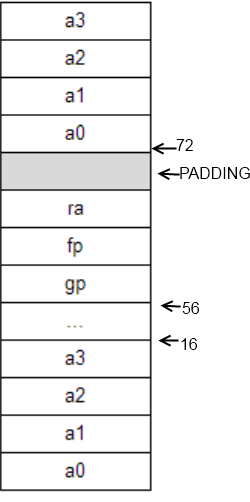
\includegraphics[height=0.50\textwidth]{ABI.png}
		\end{center}
		\caption{Stack frame generado} \label{Figura 1}
	\end{figure}
	Se ve en la figura que LTA mide 40 bytes. El tamaño no fue arbitrario si no que se tuvieron en cuenta las variables locales que se tendrían que almacenar.
	Para imprimir numeros a archivos se uso un procedimiento tambien hecho en assembly llamado \texttt{write\_int.S}
	Para debuggear se usaron llamadas de MIPS a C de la función printf en versiones para enteros y floats, las mismas se pueden ver al final del código adjunto como \texttt{miprintf} y \texttt{printff} respectivamente.
	
	\emph{Nota:} El programa en la versión actual contiene un bug que no permite la correcta impresión del brillo de los pixeles.  


	
	
\section{Corridas de prueba y Mediciones}



\section{Conclusiones}	
	Como se enuncia en el objetivo de este trabajo práctico, aprendimos a instalar y manejar el GxEmul, a realizar transferencias de archivos en Linux, así como también compilar y ejecutar programas en el NetBSD. Por otro lado,  aprendimos a manejar y escribir informes en \LaTeX{}.
	De este modo, estamos preparados para que en los próximos trabajos prácticos, nos aboquemos directamente al desarrollo de los mismos.


\newpage 
\section{Código}
\subsection{mips32\_plot.S}
\lstset{ language = [x86masm]assembler }
\lstinputlisting[label=maincode]{../mips32_plot.S}

\newpage 
\subsection{write\_int.S}
\lstset{ language = [x86masm]assembler }
\lstinputlisting[label=maincode]{../write_int.S}


\newpage 

\end{document}
